\documentclass[twoside]{book}

% Packages required by doxygen
\usepackage{fixltx2e}
\usepackage{calc}
\usepackage{doxygen}
\usepackage[export]{adjustbox} % also loads graphicx
\usepackage{graphicx}
\usepackage[utf8]{inputenc}
\usepackage{makeidx}
\usepackage{multicol}
\usepackage{multirow}
\PassOptionsToPackage{warn}{textcomp}
\usepackage{textcomp}
\usepackage[nointegrals]{wasysym}
\usepackage[table]{xcolor}

% Font selection
\usepackage[T1]{fontenc}
\usepackage[scaled=.90]{helvet}
\usepackage{courier}
\usepackage{amssymb}
\usepackage{sectsty}
\renewcommand{\familydefault}{\sfdefault}
\allsectionsfont{%
  \fontseries{bc}\selectfont%
  \color{darkgray}%
}
\renewcommand{\DoxyLabelFont}{%
  \fontseries{bc}\selectfont%
  \color{darkgray}%
}
\newcommand{\+}{\discretionary{\mbox{\scriptsize$\hookleftarrow$}}{}{}}

% Page & text layout
\usepackage{geometry}
\geometry{%
  a4paper,%
  top=2.5cm,%
  bottom=2.5cm,%
  left=2.5cm,%
  right=2.5cm%
}
\tolerance=750
\hfuzz=15pt
\hbadness=750
\setlength{\emergencystretch}{15pt}
\setlength{\parindent}{0cm}
\setlength{\parskip}{3ex plus 2ex minus 2ex}
\makeatletter
\renewcommand{\paragraph}{%
  \@startsection{paragraph}{4}{0ex}{-1.0ex}{1.0ex}{%
    \normalfont\normalsize\bfseries\SS@parafont%
  }%
}
\renewcommand{\subparagraph}{%
  \@startsection{subparagraph}{5}{0ex}{-1.0ex}{1.0ex}{%
    \normalfont\normalsize\bfseries\SS@subparafont%
  }%
}
\makeatother

% Headers & footers
\usepackage{fancyhdr}
\pagestyle{fancyplain}
\fancyhead[LE]{\fancyplain{}{\bfseries\thepage}}
\fancyhead[CE]{\fancyplain{}{}}
\fancyhead[RE]{\fancyplain{}{\bfseries\leftmark}}
\fancyhead[LO]{\fancyplain{}{\bfseries\rightmark}}
\fancyhead[CO]{\fancyplain{}{}}
\fancyhead[RO]{\fancyplain{}{\bfseries\thepage}}
\fancyfoot[LE]{\fancyplain{}{}}
\fancyfoot[CE]{\fancyplain{}{}}
\fancyfoot[RE]{\fancyplain{}{\bfseries\scriptsize Generated by Doxygen }}
\fancyfoot[LO]{\fancyplain{}{\bfseries\scriptsize Generated by Doxygen }}
\fancyfoot[CO]{\fancyplain{}{}}
\fancyfoot[RO]{\fancyplain{}{}}
\renewcommand{\footrulewidth}{0.4pt}
\renewcommand{\chaptermark}[1]{%
  \markboth{#1}{}%
}
\renewcommand{\sectionmark}[1]{%
  \markright{\thesection\ #1}%
}

% Indices & bibliography
\usepackage{natbib}
\usepackage[titles]{tocloft}
\setcounter{tocdepth}{3}
\setcounter{secnumdepth}{5}
\makeindex

% Hyperlinks (required, but should be loaded last)
\usepackage{ifpdf}
\ifpdf
  \usepackage[pdftex,pagebackref=true]{hyperref}
\else
  \usepackage[ps2pdf,pagebackref=true]{hyperref}
\fi
\hypersetup{%
  colorlinks=true,%
  linkcolor=blue,%
  citecolor=blue,%
  unicode%
}

% Custom commands
\newcommand{\clearemptydoublepage}{%
  \newpage{\pagestyle{empty}\cleardoublepage}%
}

\usepackage{caption}
\captionsetup{labelsep=space,justification=centering,font={bf},singlelinecheck=off,skip=4pt,position=top}

%===== C O N T E N T S =====

\begin{document}

% Titlepage & ToC
\hypersetup{pageanchor=false,
             bookmarksnumbered=true,
             pdfencoding=unicode
            }
\pagenumbering{alph}
\begin{titlepage}
\vspace*{7cm}
\begin{center}%
{\Large Solar system }\\
\vspace*{1cm}
{\large Generated by Doxygen 1.8.13}\\
\end{center}
\end{titlepage}
\clearemptydoublepage
\pagenumbering{roman}
\tableofcontents
\clearemptydoublepage
\pagenumbering{arabic}
\hypersetup{pageanchor=true}

%--- Begin generated contents ---
\chapter{File Index}
\section{File List}
Here is a list of all documented files with brief descriptions\+:\begin{DoxyCompactList}
\item\contentsline{section}{src/\hyperlink{solar__system_8c}{solar\+\_\+system.\+c} \\*Interactive solar system~\newline
Uses the following reusable code\+: }{\pageref{solar__system_8c}}{}
\end{DoxyCompactList}

\chapter{File Documentation}
\hypertarget{solar__system_8c}{}\section{src/solar\+\_\+system.c File Reference}
\label{solar__system_8c}\index{src/solar\+\_\+system.\+c@{src/solar\+\_\+system.\+c}}


Interactive solar system~\newline
Uses the following reusable code\+:  


{\ttfamily \#include $<$stdio.\+h$>$}\newline
{\ttfamily \#include $<$stdlib.\+h$>$}\newline
{\ttfamily \#include $<$string.\+h$>$}\newline
{\ttfamily \#include $<$math.\+h$>$}\newline
{\ttfamily \#include \char`\"{}Micro\+Glut.\+h\char`\"{}}\newline
{\ttfamily \#include \char`\"{}G\+L\+\_\+utilities.\+h\char`\"{}}\newline
{\ttfamily \#include \char`\"{}Vector\+Utils3.\+h\char`\"{}}\newline
{\ttfamily \#include \char`\"{}loadobj.\+h\char`\"{}}\newline
{\ttfamily \#include \char`\"{}Load\+T\+G\+A.\+h\char`\"{}}\newline
Include dependency graph for solar\+\_\+system.\+c\+:\nopagebreak
\begin{figure}[H]
\begin{center}
\leavevmode
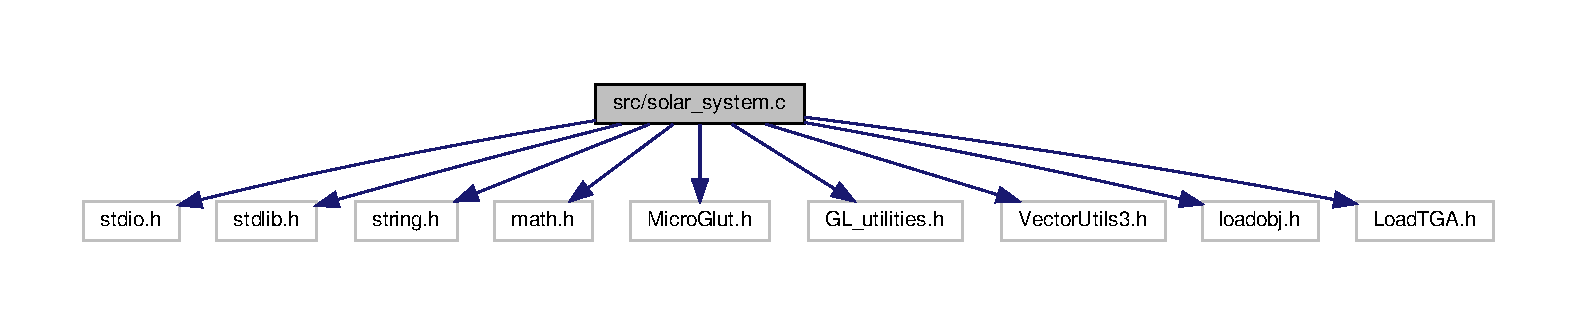
\includegraphics[width=350pt]{solar__system_8c__incl}
\end{center}
\end{figure}
\subsection*{Macros}
\begin{DoxyCompactItemize}
\item 
\mbox{\Hypertarget{solar__system_8c_a30daf1d024fa1130b3291391a3b0773d}\label{solar__system_8c_a30daf1d024fa1130b3291391a3b0773d}} 
\#define \hyperlink{solar__system_8c_a30daf1d024fa1130b3291391a3b0773d}{R\+O\+T\+A\+T\+I\+O\+N\+\_\+\+D\+E\+G\+R\+EE}~M\+\_\+\+PI/100
\begin{DoxyCompactList}\small\item\em Rotation degree for rocket movement. \end{DoxyCompactList}\end{DoxyCompactItemize}
\subsection*{Functions}
\begin{DoxyCompactItemize}
\item 
mat4 \hyperlink{solar__system_8c_a66633a93f818d5ef20e6e6243164667b}{Set\+Matrix4} (G\+Lfloat p0, G\+Lfloat p1, G\+Lfloat p2, G\+Lfloat p3, G\+Lfloat p4, G\+Lfloat p5, G\+Lfloat p6, G\+Lfloat p7, G\+Lfloat p8, G\+Lfloat p9, G\+Lfloat p10, G\+Lfloat p11, G\+Lfloat p12, G\+Lfloat p13, G\+Lfloat p14, G\+Lfloat p15)
\begin{DoxyCompactList}\small\item\em Return a 4 by 4 matrix taking the arguments as matrix numbers. \end{DoxyCompactList}\item 
\mbox{\Hypertarget{solar__system_8c_a052a3c016cd0af4daa901f62769a2cf9}\label{solar__system_8c_a052a3c016cd0af4daa901f62769a2cf9}} 
void \hyperlink{solar__system_8c_a052a3c016cd0af4daa901f62769a2cf9}{load\+Textures} ()
\begin{DoxyCompactList}\small\item\em Load and active texture for the cubemap, planets, satellite and rocket. \end{DoxyCompactList}\item 
float \hyperlink{solar__system_8c_a7a54549f44b760e639bc2fe9afec4541}{Radius\+Obj} (Model $\ast$m, float scalar)
\begin{DoxyCompactList}\small\item\em Calculate the radius of a scaled model. \end{DoxyCompactList}\item 
void \hyperlink{solar__system_8c_a9691649c7fc2dcb79da05755360dde14}{Collision\+Detection} (float radius\+\_\+sphere)
\begin{DoxyCompactList}\small\item\em Detect if there is a collision between the rocket and a sphere. In that case, the rocket move arouond the sphere as it was landing on it. \end{DoxyCompactList}\item 
void \hyperlink{solar__system_8c_a6e07312b3a723a9e37e9c5df2a065f2e}{keyboard} (unsigned char c, int x, int y)
\begin{DoxyCompactList}\small\item\em Control the camera and rocket movement with the keyboard. \end{DoxyCompactList}\item 
void \hyperlink{solar__system_8c_a23a1d350756179919bf2c2c15d6764d0}{timer} (int i)
\begin{DoxyCompactList}\small\item\em Orders a new call to the display function plus starts the next round with the timer. \end{DoxyCompactList}\item 
\mbox{\Hypertarget{solar__system_8c_a02fd73d861ef2e4aabb38c0c9ff82947}\label{solar__system_8c_a02fd73d861ef2e4aabb38c0c9ff82947}} 
void \hyperlink{solar__system_8c_a02fd73d861ef2e4aabb38c0c9ff82947}{init} ()
\begin{DoxyCompactList}\small\item\em Initialize some global variables and send projection matrix to the vertex shaders. \end{DoxyCompactList}\item 
\mbox{\Hypertarget{solar__system_8c_a4ea013001a5fb47853d0fab8f8de35cd}\label{solar__system_8c_a4ea013001a5fb47853d0fab8f8de35cd}} 
void \hyperlink{solar__system_8c_a4ea013001a5fb47853d0fab8f8de35cd}{display} (void)
\begin{DoxyCompactList}\small\item\em Redisplay the current window. \end{DoxyCompactList}\item 
int \hyperlink{solar__system_8c_a3c04138a5bfe5d72780bb7e82a18e627}{main} (int argc, char $\ast$$\ast$argv)
\begin{DoxyCompactList}\small\item\em Main program. \end{DoxyCompactList}\end{DoxyCompactItemize}
\subsection*{Variables}
\begin{DoxyCompactItemize}
\item 
\mbox{\Hypertarget{solar__system_8c_a353688eb72ea0b8e3b949cc7b9158de2}\label{solar__system_8c_a353688eb72ea0b8e3b949cc7b9158de2}} 
G\+Lfloat \hyperlink{solar__system_8c_a353688eb72ea0b8e3b949cc7b9158de2}{vertices} \mbox{[}6\mbox{]}\mbox{[}6 $\ast$3\mbox{]}
\begin{DoxyCompactList}\small\item\em Vertices positons of the skybox. \end{DoxyCompactList}\item 
\mbox{\Hypertarget{solar__system_8c_acebd6c45998e832df946feaaeb1197c1}\label{solar__system_8c_acebd6c45998e832df946feaaeb1197c1}} 
G\+Lfloat \hyperlink{solar__system_8c_acebd6c45998e832df946feaaeb1197c1}{texcoord} \mbox{[}6\mbox{]}\mbox{[}6 $\ast$2\mbox{]}
\begin{DoxyCompactList}\small\item\em Texture coordinate of the skybox. \end{DoxyCompactList}\item 
G\+Luint \hyperlink{solar__system_8c_a7e4c4ff2fd2ccd61809c3acd3c5fb6b1}{indices} \mbox{[}6\mbox{]}\mbox{[}6\mbox{]}
\begin{DoxyCompactList}\small\item\em Indices of the skybox. \end{DoxyCompactList}\item 
char $\ast$ \hyperlink{solar__system_8c_ab6d5b92c58f3da54ae510f8978d63433}{cubemap\+Texture\+File\+Name} \mbox{[}6\mbox{]}
\begin{DoxyCompactList}\small\item\em File names of the 6 cubemap textures. \end{DoxyCompactList}\item 
char $\ast$ \hyperlink{solar__system_8c_ad546c6a599e1a97315305b4d8df165de}{models\+Texture\+File\+Name} \mbox{[}11\mbox{]}
\begin{DoxyCompactList}\small\item\em File names of the planets, satellite and rocket textures. \end{DoxyCompactList}\item 
char $\ast$ \hyperlink{solar__system_8c_a312a2aedf1b912f5e7b5c4964956af8e}{models\+File\+Name} \mbox{[}2\mbox{]}
\begin{DoxyCompactList}\small\item\em File names of the 2 models (sphere and rocket) \end{DoxyCompactList}\item 
\mbox{\Hypertarget{solar__system_8c_abfa0eb2dad4e26b75086e8a2a8975259}\label{solar__system_8c_abfa0eb2dad4e26b75086e8a2a8975259}} 
Texture\+Data \hyperlink{solar__system_8c_abfa0eb2dad4e26b75086e8a2a8975259}{cubemap\+\_\+texture} \mbox{[}6\mbox{]}
\begin{DoxyCompactList}\small\item\em Texture data for the cubemap. \end{DoxyCompactList}\item 
\mbox{\Hypertarget{solar__system_8c_a94d099f138a7b9ac841b0dfa9069d382}\label{solar__system_8c_a94d099f138a7b9ac841b0dfa9069d382}} 
Texture\+Data \hyperlink{solar__system_8c_a94d099f138a7b9ac841b0dfa9069d382}{satellites\+\_\+texture} \mbox{[}10\mbox{]}
\begin{DoxyCompactList}\small\item\em Planets and satellites texture data for the planets and satellite. \end{DoxyCompactList}\item 
\mbox{\Hypertarget{solar__system_8c_aa1c5b2f3ecbfd4fcfc857f3b8f71bf92}\label{solar__system_8c_aa1c5b2f3ecbfd4fcfc857f3b8f71bf92}} 
Texture\+Data \hyperlink{solar__system_8c_aa1c5b2f3ecbfd4fcfc857f3b8f71bf92}{rocket\+\_\+texture}
\begin{DoxyCompactList}\small\item\em Rocket texture data. \end{DoxyCompactList}\item 
\mbox{\Hypertarget{solar__system_8c_a31269ba6fb67d3cb0cc9dec3cd237b2a}\label{solar__system_8c_a31269ba6fb67d3cb0cc9dec3cd237b2a}} 
mat4 \hyperlink{solar__system_8c_a31269ba6fb67d3cb0cc9dec3cd237b2a}{world\+To\+View\+Matrix}
\begin{DoxyCompactList}\small\item\em World-\/to-\/view matrix. \end{DoxyCompactList}\item 
\mbox{\Hypertarget{solar__system_8c_aa6307af2cc42a4b18c3a1d7e102af31c}\label{solar__system_8c_aa6307af2cc42a4b18c3a1d7e102af31c}} 
mat4 \hyperlink{solar__system_8c_aa6307af2cc42a4b18c3a1d7e102af31c}{projection\+Matrix}
\begin{DoxyCompactList}\small\item\em Projection matrix. \end{DoxyCompactList}\item 
\mbox{\Hypertarget{solar__system_8c_af012aa3f3b204456f0d53e990eef633c}\label{solar__system_8c_af012aa3f3b204456f0d53e990eef633c}} 
mat4 \hyperlink{solar__system_8c_af012aa3f3b204456f0d53e990eef633c}{model\+To\+World\+Matrix\+Sun}
\begin{DoxyCompactList}\small\item\em Sun model-\/to-\/world matrix. \end{DoxyCompactList}\item 
\mbox{\Hypertarget{solar__system_8c_a9141e67b4745ec54e597ea449c9763dd}\label{solar__system_8c_a9141e67b4745ec54e597ea449c9763dd}} 
mat4 \hyperlink{solar__system_8c_a9141e67b4745ec54e597ea449c9763dd}{model\+To\+World\+Matrix\+Planet}
\begin{DoxyCompactList}\small\item\em Planets model-\/to-\/world matrix. \end{DoxyCompactList}\item 
\mbox{\Hypertarget{solar__system_8c_a5d2494b9d6905b842691e8244303cc51}\label{solar__system_8c_a5d2494b9d6905b842691e8244303cc51}} 
mat4 \hyperlink{solar__system_8c_a5d2494b9d6905b842691e8244303cc51}{model\+To\+World\+Matrix\+Satellite}
\begin{DoxyCompactList}\small\item\em Satellites model-\/to-\/world matrix. \end{DoxyCompactList}\item 
\mbox{\Hypertarget{solar__system_8c_ac2ba7075888d380df017a88ac6926bd4}\label{solar__system_8c_ac2ba7075888d380df017a88ac6926bd4}} 
mat4 \hyperlink{solar__system_8c_ac2ba7075888d380df017a88ac6926bd4}{model\+To\+World\+Matrix\+Rocket}
\begin{DoxyCompactList}\small\item\em Rocket model-\/to-\/world matrix. \end{DoxyCompactList}\item 
\mbox{\Hypertarget{solar__system_8c_a27d8510c93324412d38a888eddee2852}\label{solar__system_8c_a27d8510c93324412d38a888eddee2852}} 
G\+Luint \hyperlink{solar__system_8c_a27d8510c93324412d38a888eddee2852}{program}
\begin{DoxyCompactList}\small\item\em cm shaders program \end{DoxyCompactList}\item 
\mbox{\Hypertarget{solar__system_8c_aa2b3544824cac9248e4ef5f8236bfb36}\label{solar__system_8c_aa2b3544824cac9248e4ef5f8236bfb36}} 
G\+Luint \hyperlink{solar__system_8c_aa2b3544824cac9248e4ef5f8236bfb36}{texprogram}
\begin{DoxyCompactList}\small\item\em tex shaders program \end{DoxyCompactList}\item 
\mbox{\Hypertarget{solar__system_8c_aada36b74c979c3211a21f41014210846}\label{solar__system_8c_aada36b74c979c3211a21f41014210846}} 
Model $\ast$ \hyperlink{solar__system_8c_aada36b74c979c3211a21f41014210846}{model} \mbox{[}2\mbox{]}
\begin{DoxyCompactList}\small\item\em obj models (sphere and rocket) \end{DoxyCompactList}\item 
\mbox{\Hypertarget{solar__system_8c_a37b709b18b87dc6180189e47a04198af}\label{solar__system_8c_a37b709b18b87dc6180189e47a04198af}} 
Model $\ast$ \hyperlink{solar__system_8c_a37b709b18b87dc6180189e47a04198af}{box} \mbox{[}6\mbox{]}
\begin{DoxyCompactList}\small\item\em skybox models (left, right, up, down, back and front) \end{DoxyCompactList}\item 
\mbox{\Hypertarget{solar__system_8c_ad657cb4b373120f4f218bdc824a67b42}\label{solar__system_8c_ad657cb4b373120f4f218bdc824a67b42}} 
G\+Lfloat \hyperlink{solar__system_8c_ad657cb4b373120f4f218bdc824a67b42}{rotation\+\_\+planet}
\begin{DoxyCompactList}\small\item\em Rotation speed of the planets. \end{DoxyCompactList}\item 
\mbox{\Hypertarget{solar__system_8c_abc5ab083ebc139fcf918b3cb06039294}\label{solar__system_8c_abc5ab083ebc139fcf918b3cb06039294}} 
G\+Lfloat \hyperlink{solar__system_8c_abc5ab083ebc139fcf918b3cb06039294}{translation\+\_\+planet}
\begin{DoxyCompactList}\small\item\em Translation speed of the planets. \end{DoxyCompactList}\item 
\mbox{\Hypertarget{solar__system_8c_a753b028c8c9555cc920367e4d5b2bcd7}\label{solar__system_8c_a753b028c8c9555cc920367e4d5b2bcd7}} 
G\+Lfloat \hyperlink{solar__system_8c_a753b028c8c9555cc920367e4d5b2bcd7}{translation\+\_\+satellite}
\begin{DoxyCompactList}\small\item\em Translation speed of the satellites. \end{DoxyCompactList}\item 
\mbox{\Hypertarget{solar__system_8c_a2219a4c5bf82e8b0d217c8bd7d4fcb53}\label{solar__system_8c_a2219a4c5bf82e8b0d217c8bd7d4fcb53}} 
vec3 \hyperlink{solar__system_8c_a2219a4c5bf82e8b0d217c8bd7d4fcb53}{sun\+\_\+position}
\begin{DoxyCompactList}\small\item\em Sun position. \end{DoxyCompactList}\item 
G\+Lfloat \hyperlink{solar__system_8c_ada0715c147a822226e36ded5de4de06b}{distance\+\_\+to\+\_\+sun} \mbox{[}8\mbox{]} = \{10, 30, 50, 70, 90, 110, 120, 150\}
\begin{DoxyCompactList}\small\item\em Relation between index and planets\textquotesingle{} name. \end{DoxyCompactList}\item 
\mbox{\Hypertarget{solar__system_8c_a4e3b9983e153f0b2a7e1e68272f2bf27}\label{solar__system_8c_a4e3b9983e153f0b2a7e1e68272f2bf27}} 
G\+Lfloat \hyperlink{solar__system_8c_a4e3b9983e153f0b2a7e1e68272f2bf27}{planet\+\_\+size} \mbox{[}8\mbox{]} = \{0.\+2, 0.\+5, 1, 1, 3, 3, 2, 2\}
\begin{DoxyCompactList}\small\item\em Planet\textquotesingle{}s size. \end{DoxyCompactList}\item 
\mbox{\Hypertarget{solar__system_8c_a617a02922ffc00a2a75923b6e652817c}\label{solar__system_8c_a617a02922ffc00a2a75923b6e652817c}} 
G\+Lfloat \hyperlink{solar__system_8c_a617a02922ffc00a2a75923b6e652817c}{z\+\_\+deviaton} \mbox{[}8\mbox{]} = \{-\/1, 1, -\/1, 1, -\/1, 1, -\/1, 1\}
\begin{DoxyCompactList}\small\item\em Planet\textquotesingle{}s Z deviation from the sun. \end{DoxyCompactList}\item 
\mbox{\Hypertarget{solar__system_8c_aa0f01bce4c98f2c7c59aabf7eb942694}\label{solar__system_8c_aa0f01bce4c98f2c7c59aabf7eb942694}} 
G\+Lfloat \hyperlink{solar__system_8c_aa0f01bce4c98f2c7c59aabf7eb942694}{x\+\_\+deviation} \mbox{[}8\mbox{]} = \{1, -\/1, 1, -\/1, 1, -\/1, 1, -\/1\}
\begin{DoxyCompactList}\small\item\em Planet\textquotesingle{}s X deviation from the sun. \end{DoxyCompactList}\item 
\mbox{\Hypertarget{solar__system_8c_af4aa7c841d8f18a992cecabb3c63f792}\label{solar__system_8c_af4aa7c841d8f18a992cecabb3c63f792}} 
vec3 \hyperlink{solar__system_8c_af4aa7c841d8f18a992cecabb3c63f792}{position\+\_\+rocket}
\begin{DoxyCompactList}\small\item\em Rocket position. \end{DoxyCompactList}\item 
\mbox{\Hypertarget{solar__system_8c_a27d548e67de8acbd6bef1e08bb36ef95}\label{solar__system_8c_a27d548e67de8acbd6bef1e08bb36ef95}} 
vec3 \hyperlink{solar__system_8c_a27d548e67de8acbd6bef1e08bb36ef95}{position\+\_\+camera}
\begin{DoxyCompactList}\small\item\em Camera position. \end{DoxyCompactList}\item 
\mbox{\Hypertarget{solar__system_8c_aaf14660b34613a15ed0e5a75239e0c9b}\label{solar__system_8c_aaf14660b34613a15ed0e5a75239e0c9b}} 
vec3 \hyperlink{solar__system_8c_aaf14660b34613a15ed0e5a75239e0c9b}{camera\+Vector\+General}
\begin{DoxyCompactList}\small\item\em look\+At camera vector parameter for general view \end{DoxyCompactList}\item 
\mbox{\Hypertarget{solar__system_8c_af7cf90897c413216bfbba726682428bb}\label{solar__system_8c_af7cf90897c413216bfbba726682428bb}} 
vec3 \hyperlink{solar__system_8c_af7cf90897c413216bfbba726682428bb}{view\+Vector\+General}
\begin{DoxyCompactList}\small\item\em look\+At view vector parameter for general view \end{DoxyCompactList}\item 
\mbox{\Hypertarget{solar__system_8c_a55a4667d7a30d616251f98764fb68e16}\label{solar__system_8c_a55a4667d7a30d616251f98764fb68e16}} 
vec3 \hyperlink{solar__system_8c_a55a4667d7a30d616251f98764fb68e16}{up\+Vector\+General}
\begin{DoxyCompactList}\small\item\em look\+At up vector parameter for general view \end{DoxyCompactList}\item 
\mbox{\Hypertarget{solar__system_8c_ab47b818590551b1663a0cd5c060d92b6}\label{solar__system_8c_ab47b818590551b1663a0cd5c060d92b6}} 
G\+Lfloat \hyperlink{solar__system_8c_ab47b818590551b1663a0cd5c060d92b6}{angle} = 0.\+0
\begin{DoxyCompactList}\small\item\em Rotation angle over XZ plane in general view. \end{DoxyCompactList}\item 
\mbox{\Hypertarget{solar__system_8c_af001c03dcf73b455df403386222f2e83}\label{solar__system_8c_af001c03dcf73b455df403386222f2e83}} 
G\+Lint \hyperlink{solar__system_8c_af001c03dcf73b455df403386222f2e83}{cam} = 0
\begin{DoxyCompactList}\small\item\em 0 = general view, 1 = rocket view \end{DoxyCompactList}\item 
\mbox{\Hypertarget{solar__system_8c_a13cc8879927ac10ae7b03266d82647b4}\label{solar__system_8c_a13cc8879927ac10ae7b03266d82647b4}} 
vec3 \hyperlink{solar__system_8c_a13cc8879927ac10ae7b03266d82647b4}{forward\+Vector}
\begin{DoxyCompactList}\small\item\em Rocket forward vector. \end{DoxyCompactList}\item 
\mbox{\Hypertarget{solar__system_8c_ae4e35efd9ff02a4ad63abe94c5684402}\label{solar__system_8c_ae4e35efd9ff02a4ad63abe94c5684402}} 
vec3 \hyperlink{solar__system_8c_ae4e35efd9ff02a4ad63abe94c5684402}{right\+Vector}
\begin{DoxyCompactList}\small\item\em Rocket right vector. \end{DoxyCompactList}\item 
\mbox{\Hypertarget{solar__system_8c_aa99831808e17a6accfe5a3bf76b732aa}\label{solar__system_8c_aa99831808e17a6accfe5a3bf76b732aa}} 
vec3 \hyperlink{solar__system_8c_aa99831808e17a6accfe5a3bf76b732aa}{up\+Vector}
\begin{DoxyCompactList}\small\item\em Rocket up vector. \end{DoxyCompactList}\item 
\mbox{\Hypertarget{solar__system_8c_afb77920451f978c6664d5a9e559bae1d}\label{solar__system_8c_afb77920451f978c6664d5a9e559bae1d}} 
mat4 \hyperlink{solar__system_8c_afb77920451f978c6664d5a9e559bae1d}{rotation\+\_\+matrix}
\begin{DoxyCompactList}\small\item\em Rocket rotation matrix. \end{DoxyCompactList}\item 
\mbox{\Hypertarget{solar__system_8c_a6a0004161c8412275239ae6dfc2623df}\label{solar__system_8c_a6a0004161c8412275239ae6dfc2623df}} 
vec3 \hyperlink{solar__system_8c_a6a0004161c8412275239ae6dfc2623df}{camera\+Direction\+Vector}
\begin{DoxyCompactList}\small\item\em Vector from the rocket to the camera. \end{DoxyCompactList}\item 
\mbox{\Hypertarget{solar__system_8c_a58459d4856813c1cede73d8fd35a4c17}\label{solar__system_8c_a58459d4856813c1cede73d8fd35a4c17}} 
vec3 \hyperlink{solar__system_8c_a58459d4856813c1cede73d8fd35a4c17}{sphere\+\_\+position}
\begin{DoxyCompactList}\small\item\em Position if the sphere. \end{DoxyCompactList}\item 
\mbox{\Hypertarget{solar__system_8c_a39cc10153997b3e34c3e2c48e97bb0f0}\label{solar__system_8c_a39cc10153997b3e34c3e2c48e97bb0f0}} 
vec3 \hyperlink{solar__system_8c_a39cc10153997b3e34c3e2c48e97bb0f0}{sphere\+Forward\+Vector}
\begin{DoxyCompactList}\small\item\em New forward vector of the rocket after a collision. \end{DoxyCompactList}\item 
\mbox{\Hypertarget{solar__system_8c_a0e174967f63f40c355f0b3246c7c3574}\label{solar__system_8c_a0e174967f63f40c355f0b3246c7c3574}} 
G\+Lfloat \hyperlink{solar__system_8c_a0e174967f63f40c355f0b3246c7c3574}{radius\+\_\+satellite}
\begin{DoxyCompactList}\small\item\em Satellite\textquotesingle{}s radius. \end{DoxyCompactList}\item 
\mbox{\Hypertarget{solar__system_8c_ad5938eac9210f56048873a5687291d87}\label{solar__system_8c_ad5938eac9210f56048873a5687291d87}} 
G\+Lfloat \hyperlink{solar__system_8c_ad5938eac9210f56048873a5687291d87}{radius\+\_\+rocket}
\begin{DoxyCompactList}\small\item\em Rocket\textquotesingle{}s radius. \end{DoxyCompactList}\item 
\mbox{\Hypertarget{solar__system_8c_acc3557de6324478d449e05736215bd33}\label{solar__system_8c_acc3557de6324478d449e05736215bd33}} 
G\+Lfloat \hyperlink{solar__system_8c_acc3557de6324478d449e05736215bd33}{radius\+\_\+sun}
\begin{DoxyCompactList}\small\item\em Sun\textquotesingle{}s radius. \end{DoxyCompactList}\item 
\mbox{\Hypertarget{solar__system_8c_a913632569763ab145864dc5e6d1500a4}\label{solar__system_8c_a913632569763ab145864dc5e6d1500a4}} 
G\+Lfloat \hyperlink{solar__system_8c_a913632569763ab145864dc5e6d1500a4}{radius\+\_\+planets} \mbox{[}8\mbox{]}
\begin{DoxyCompactList}\small\item\em Plantes\textquotesingle{} radius. \end{DoxyCompactList}\item 
\mbox{\Hypertarget{solar__system_8c_a0b2f45f339a9a2473f545d215418f3ee}\label{solar__system_8c_a0b2f45f339a9a2473f545d215418f3ee}} 
vec3 \hyperlink{solar__system_8c_a0b2f45f339a9a2473f545d215418f3ee}{normal\+\_\+vector}
\begin{DoxyCompactList}\small\item\em Normal vector for sphere\+Forward\+Vector calculation. \end{DoxyCompactList}\item 
\mbox{\Hypertarget{solar__system_8c_a039d7c51c60eb3409de8474a305e7f5b}\label{solar__system_8c_a039d7c51c60eb3409de8474a305e7f5b}} 
vec3 \hyperlink{solar__system_8c_a039d7c51c60eb3409de8474a305e7f5b}{tangent\+\_\+vector}
\begin{DoxyCompactList}\small\item\em Tangent vector for sphere\+Forward\+Vector calculation. \end{DoxyCompactList}\end{DoxyCompactItemize}


\subsection{Detailed Description}
Interactive solar system~\newline
Uses the following reusable code\+: 


\begin{DoxyItemize}
\item G\+L\+\_\+utilities (shader loader)
\item Micro\+G\+L\+UT (G\+L\+UT replacement)~\newline

\item Vector\+Utils3 (vector/matrix code)
\item loadobj (limited O\+BJ model loader)
\item Load\+T\+GA (loader for textures saved as T\+GA files)
\end{DoxyItemize}

\begin{DoxyAuthor}{Author}
Roberto Corrochano Piqueras (robco726) 

Sergio García Prados (serga155) 
\end{DoxyAuthor}
\begin{DoxyDate}{Date}
13/05/2019 
\end{DoxyDate}


\subsection{Function Documentation}
\mbox{\Hypertarget{solar__system_8c_a9691649c7fc2dcb79da05755360dde14}\label{solar__system_8c_a9691649c7fc2dcb79da05755360dde14}} 
\index{solar\+\_\+system.\+c@{solar\+\_\+system.\+c}!Collision\+Detection@{Collision\+Detection}}
\index{Collision\+Detection@{Collision\+Detection}!solar\+\_\+system.\+c@{solar\+\_\+system.\+c}}
\subsubsection{\texorpdfstring{Collision\+Detection()}{CollisionDetection()}}
{\footnotesize\ttfamily void Collision\+Detection (\begin{DoxyParamCaption}\item[{float}]{radius\+\_\+sphere }\end{DoxyParamCaption})}



Detect if there is a collision between the rocket and a sphere. In that case, the rocket move arouond the sphere as it was landing on it. 


\begin{DoxyParams}{Parameters}
{\em radius\+\_\+sphere} & Radius of the sphere which the rocket could collide with \\
\hline
\end{DoxyParams}
\begin{DoxyPrecond}{Precondition}
radius\+\_\+sphere should be greater than 0 
\end{DoxyPrecond}


Definition at line 299 of file solar\+\_\+system.\+c.

\mbox{\Hypertarget{solar__system_8c_a6e07312b3a723a9e37e9c5df2a065f2e}\label{solar__system_8c_a6e07312b3a723a9e37e9c5df2a065f2e}} 
\index{solar\+\_\+system.\+c@{solar\+\_\+system.\+c}!keyboard@{keyboard}}
\index{keyboard@{keyboard}!solar\+\_\+system.\+c@{solar\+\_\+system.\+c}}
\subsubsection{\texorpdfstring{keyboard()}{keyboard()}}
{\footnotesize\ttfamily void keyboard (\begin{DoxyParamCaption}\item[{unsigned char}]{c,  }\item[{int}]{x,  }\item[{int}]{y }\end{DoxyParamCaption})}



Control the camera and rocket movement with the keyboard. 


\begin{DoxyParams}{Parameters}
{\em c} & Key pressed \\
\hline
{\em x} & Mouse X location in window relative coordinates when the key was pressed \\
\hline
{\em y} & Mouse Y location in window relative coordinates when the key was pressed \\
\hline
\end{DoxyParams}


Definition at line 318 of file solar\+\_\+system.\+c.

\mbox{\Hypertarget{solar__system_8c_a3c04138a5bfe5d72780bb7e82a18e627}\label{solar__system_8c_a3c04138a5bfe5d72780bb7e82a18e627}} 
\index{solar\+\_\+system.\+c@{solar\+\_\+system.\+c}!main@{main}}
\index{main@{main}!solar\+\_\+system.\+c@{solar\+\_\+system.\+c}}
\subsubsection{\texorpdfstring{main()}{main()}}
{\footnotesize\ttfamily int main (\begin{DoxyParamCaption}\item[{int}]{argc,  }\item[{char $\ast$$\ast$}]{argv }\end{DoxyParamCaption})}



Main program. 


\begin{DoxyParams}{Parameters}
{\em argc} & Number of arguments \\
\hline
{\em argv} & Pointer to the arguments \\
\hline
\end{DoxyParams}


Definition at line 586 of file solar\+\_\+system.\+c.

\mbox{\Hypertarget{solar__system_8c_a7a54549f44b760e639bc2fe9afec4541}\label{solar__system_8c_a7a54549f44b760e639bc2fe9afec4541}} 
\index{solar\+\_\+system.\+c@{solar\+\_\+system.\+c}!Radius\+Obj@{Radius\+Obj}}
\index{Radius\+Obj@{Radius\+Obj}!solar\+\_\+system.\+c@{solar\+\_\+system.\+c}}
\subsubsection{\texorpdfstring{Radius\+Obj()}{RadiusObj()}}
{\footnotesize\ttfamily float Radius\+Obj (\begin{DoxyParamCaption}\item[{Model $\ast$}]{m,  }\item[{float}]{scalar }\end{DoxyParamCaption})}



Calculate the radius of a scaled model. 


\begin{DoxyParams}{Parameters}
{\em m} & Model to calculate its radius \\
\hline
{\em scalar} & Scalar number for the model \\
\hline
\end{DoxyParams}
\begin{DoxyPrecond}{Precondition}
m should exist and be loaded 

scalar should be greater than 0 
\end{DoxyPrecond}
\begin{DoxyReturn}{Returns}
Radius of the scaled model 
\end{DoxyReturn}


Definition at line 286 of file solar\+\_\+system.\+c.

\mbox{\Hypertarget{solar__system_8c_a66633a93f818d5ef20e6e6243164667b}\label{solar__system_8c_a66633a93f818d5ef20e6e6243164667b}} 
\index{solar\+\_\+system.\+c@{solar\+\_\+system.\+c}!Set\+Matrix4@{Set\+Matrix4}}
\index{Set\+Matrix4@{Set\+Matrix4}!solar\+\_\+system.\+c@{solar\+\_\+system.\+c}}
\subsubsection{\texorpdfstring{Set\+Matrix4()}{SetMatrix4()}}
{\footnotesize\ttfamily mat4 Set\+Matrix4 (\begin{DoxyParamCaption}\item[{G\+Lfloat}]{p0,  }\item[{G\+Lfloat}]{p1,  }\item[{G\+Lfloat}]{p2,  }\item[{G\+Lfloat}]{p3,  }\item[{G\+Lfloat}]{p4,  }\item[{G\+Lfloat}]{p5,  }\item[{G\+Lfloat}]{p6,  }\item[{G\+Lfloat}]{p7,  }\item[{G\+Lfloat}]{p8,  }\item[{G\+Lfloat}]{p9,  }\item[{G\+Lfloat}]{p10,  }\item[{G\+Lfloat}]{p11,  }\item[{G\+Lfloat}]{p12,  }\item[{G\+Lfloat}]{p13,  }\item[{G\+Lfloat}]{p14,  }\item[{G\+Lfloat}]{p15 }\end{DoxyParamCaption})}



Return a 4 by 4 matrix taking the arguments as matrix numbers. 


\begin{DoxyParams}{Parameters}
{\em p0} & 0x0 element \\
\hline
{\em p1} & 0x1 element \\
\hline
{\em p2} & 0x2 element \\
\hline
{\em p3} & 0x3 element \\
\hline
{\em p4} & 1x0 element \\
\hline
{\em p5} & 1x1 element \\
\hline
{\em p6} & 1x2 element \\
\hline
{\em p7} & 1x3 element \\
\hline
{\em p8} & 2x0 element \\
\hline
{\em p9} & 2x1 element \\
\hline
{\em p10} & 2x2 element \\
\hline
{\em p11} & 2x3 element \\
\hline
{\em p12} & 3x0 element \\
\hline
{\em p13} & 3x1 element \\
\hline
{\em p14} & 3x2 element \\
\hline
{\em p15} & 3x3 element \\
\hline
\end{DoxyParams}
\begin{DoxyReturn}{Returns}
A 4x4 matrix 
\end{DoxyReturn}


Definition at line 214 of file solar\+\_\+system.\+c.

\mbox{\Hypertarget{solar__system_8c_a23a1d350756179919bf2c2c15d6764d0}\label{solar__system_8c_a23a1d350756179919bf2c2c15d6764d0}} 
\index{solar\+\_\+system.\+c@{solar\+\_\+system.\+c}!timer@{timer}}
\index{timer@{timer}!solar\+\_\+system.\+c@{solar\+\_\+system.\+c}}
\subsubsection{\texorpdfstring{timer()}{timer()}}
{\footnotesize\ttfamily void timer (\begin{DoxyParamCaption}\item[{int}]{i }\end{DoxyParamCaption})}



Orders a new call to the display function plus starts the next round with the timer. 


\begin{DoxyParams}{Parameters}
{\em i} & Value parameter to glut\+Timer\+Func \\
\hline
\end{DoxyParams}


Definition at line 389 of file solar\+\_\+system.\+c.



\subsection{Variable Documentation}
\mbox{\Hypertarget{solar__system_8c_ab6d5b92c58f3da54ae510f8978d63433}\label{solar__system_8c_ab6d5b92c58f3da54ae510f8978d63433}} 
\index{solar\+\_\+system.\+c@{solar\+\_\+system.\+c}!cubemap\+Texture\+File\+Name@{cubemap\+Texture\+File\+Name}}
\index{cubemap\+Texture\+File\+Name@{cubemap\+Texture\+File\+Name}!solar\+\_\+system.\+c@{solar\+\_\+system.\+c}}
\subsubsection{\texorpdfstring{cubemap\+Texture\+File\+Name}{cubemapTextureFileName}}
{\footnotesize\ttfamily char$\ast$ cubemap\+Texture\+File\+Name\mbox{[}6\mbox{]}}

{\bfseries Initial value\+:}
\begin{DoxyCode}
=
\{
    \textcolor{stringliteral}{"textures/purplenebula\_lf.tga"},
    \textcolor{stringliteral}{"textures/purplenebula\_rt.tga"},
    \textcolor{stringliteral}{"textures/purplenebula\_up.tga"},
    \textcolor{stringliteral}{"textures/purplenebula\_dn.tga"},
    \textcolor{stringliteral}{"textures/purplenebula\_bk.tga"},
    \textcolor{stringliteral}{"textures/purplenebula\_ft.tga"}
\}
\end{DoxyCode}


File names of the 6 cubemap textures. 



Definition at line 117 of file solar\+\_\+system.\+c.

\mbox{\Hypertarget{solar__system_8c_ada0715c147a822226e36ded5de4de06b}\label{solar__system_8c_ada0715c147a822226e36ded5de4de06b}} 
\index{solar\+\_\+system.\+c@{solar\+\_\+system.\+c}!distance\+\_\+to\+\_\+sun@{distance\+\_\+to\+\_\+sun}}
\index{distance\+\_\+to\+\_\+sun@{distance\+\_\+to\+\_\+sun}!solar\+\_\+system.\+c@{solar\+\_\+system.\+c}}
\subsubsection{\texorpdfstring{distance\+\_\+to\+\_\+sun}{distance\_to\_sun}}
{\footnotesize\ttfamily G\+Lfloat distance\+\_\+to\+\_\+sun\mbox{[}8\mbox{]} = \{10, 30, 50, 70, 90, 110, 120, 150\}}



Relation between index and planets\textquotesingle{} name. 


\begin{DoxyItemize}
\item Planet\textquotesingle{}s distance to sun (0 = Mercury, 1 = Venus, 2 = Earth, 3 = Mars, 4 = Jupiter, 5 = Saturn, 6 = Uranus, 7 = Neptune) 
\end{DoxyItemize}

Definition at line 169 of file solar\+\_\+system.\+c.

\mbox{\Hypertarget{solar__system_8c_a7e4c4ff2fd2ccd61809c3acd3c5fb6b1}\label{solar__system_8c_a7e4c4ff2fd2ccd61809c3acd3c5fb6b1}} 
\index{solar\+\_\+system.\+c@{solar\+\_\+system.\+c}!indices@{indices}}
\index{indices@{indices}!solar\+\_\+system.\+c@{solar\+\_\+system.\+c}}
\subsubsection{\texorpdfstring{indices}{indices}}
{\footnotesize\ttfamily G\+Luint indices\mbox{[}6\mbox{]}\mbox{[}6\mbox{]}}

{\bfseries Initial value\+:}
\begin{DoxyCode}
=
\{
    \{0, 2, 1, 0, 3, 2\},
    \{0, 2, 1, 0, 3, 2\},
    \{0, 2, 1, 0, 3, 2\},
    \{0, 2, 1, 0, 3, 2\},
    \{0, 2, 1, 0, 3, 2\},
    \{0, 2, 1, 0, 3, 2\}
\}
\end{DoxyCode}


Indices of the skybox. 



Definition at line 107 of file solar\+\_\+system.\+c.

\mbox{\Hypertarget{solar__system_8c_a312a2aedf1b912f5e7b5c4964956af8e}\label{solar__system_8c_a312a2aedf1b912f5e7b5c4964956af8e}} 
\index{solar\+\_\+system.\+c@{solar\+\_\+system.\+c}!models\+File\+Name@{models\+File\+Name}}
\index{models\+File\+Name@{models\+File\+Name}!solar\+\_\+system.\+c@{solar\+\_\+system.\+c}}
\subsubsection{\texorpdfstring{models\+File\+Name}{modelsFileName}}
{\footnotesize\ttfamily char$\ast$ models\+File\+Name\mbox{[}2\mbox{]}}

{\bfseries Initial value\+:}
\begin{DoxyCode}
=
\{
    \textcolor{stringliteral}{"obj/Sphere.obj"},
    \textcolor{stringliteral}{"obj/Rocket.obj"}
\}
\end{DoxyCode}


File names of the 2 models (sphere and rocket) 



Definition at line 142 of file solar\+\_\+system.\+c.

\mbox{\Hypertarget{solar__system_8c_ad546c6a599e1a97315305b4d8df165de}\label{solar__system_8c_ad546c6a599e1a97315305b4d8df165de}} 
\index{solar\+\_\+system.\+c@{solar\+\_\+system.\+c}!models\+Texture\+File\+Name@{models\+Texture\+File\+Name}}
\index{models\+Texture\+File\+Name@{models\+Texture\+File\+Name}!solar\+\_\+system.\+c@{solar\+\_\+system.\+c}}
\subsubsection{\texorpdfstring{models\+Texture\+File\+Name}{modelsTextureFileName}}
{\footnotesize\ttfamily char$\ast$ models\+Texture\+File\+Name\mbox{[}11\mbox{]}}

{\bfseries Initial value\+:}
\begin{DoxyCode}
=
\{
    \textcolor{stringliteral}{"textures/sun\_texture.tga"},
    \textcolor{stringliteral}{"textures/mercury\_texture.tga"},
    \textcolor{stringliteral}{"textures/venus\_texture.tga"},
    \textcolor{stringliteral}{"textures/earth\_texture.tga"},
    \textcolor{stringliteral}{"textures/mars\_texture.tga"},
    \textcolor{stringliteral}{"textures/jupiter\_texture.tga"},
    \textcolor{stringliteral}{"textures/saturn\_texture.tga"},
    \textcolor{stringliteral}{"textures/uranus\_texture.tga"},
    \textcolor{stringliteral}{"textures/neptune\_texture.tga"},
    \textcolor{stringliteral}{"textures/moon\_texture.tga"},
    \textcolor{stringliteral}{"textures/rocket\_texture.tga"}
\}
\end{DoxyCode}


File names of the planets, satellite and rocket textures. 



Definition at line 127 of file solar\+\_\+system.\+c.


%--- End generated contents ---

% Index
\backmatter
\newpage
\phantomsection
\clearemptydoublepage
\addcontentsline{toc}{chapter}{Index}
\printindex

\end{document}
